% ============================================================
%  CHAPTER 3 — System Design and Implementation
% ============================================================
\chapter{System Design and Implementation}
\label{ch:system}

This chapter describes the complete design and implementation of the TIAGo VLA
agent --- a system that allows a physical mobile manipulator to understand spoken
or typed commands and carry them out autonomously in the real world.
The chapter is organised as a coherent narrative that follows the flow of a
single command through the system: from the user's words all the way to a
physical action on the robot.
We first introduce the hardware platform, then describe the overall architecture,
and then go into the implementation details of each subsystem: the
perceive-reason-act loop, perception, vision-language reasoning, manipulation
and grasping, agent orchestration, and the safety architecture.

% ============================================================
\section{Hardware Platform: The TIAGo Robot}
\label{sec:hardware}
% ============================================================

All experiments and development were conducted on a \textbf{PAL Robotics TIAGo}
(Take It And Go) mobile manipulator.
TIAGo was chosen because it is the robot available in the laboratory, and its
physical design turns out to be particularly well suited to the manipulation
approach developed in this work.
Figure~\ref{fig:tiago_real} shows the complete platform with its main subsystems
labelled.

\begin{figure}[H]
  \centering
  \includegraphics[width=0.65\textwidth]{figures/TIAGo_overview.png}
  \caption{The PAL Robotics TIAGo mobile manipulator. All development and
           experiments in this work were conducted on this platform.
           Image courtesy of PAL Robotics.}
  \label{fig:tiago_real}
\end{figure}

The robot combines four mechanical subsystems.
The \textbf{omnidirectional mobile base} carries the entire structure and allows
the robot to translate and rotate in any direction without re-orientation.
It runs the ROS \texttt{move\_base} navigation stack and communicates with a 2-D
laser scanner for obstacle avoidance.
Above the base, a \textbf{prismatic torso lift} raises and lowers the upper body
along a world-Z-aligned vertical rail by up to 35\,cm.
This linear degree of freedom turns out to be the key enabling mechanism for
robust grasping, as discussed in Section~\ref{sec:manipulation}.
The 7-DOF \textbf{manipulator arm} (Figure~\ref{fig:arm_torso}) is mounted on
the torso and consists of four M90 actuator modules plus a 3-DOF wrist, giving
a total reach of approximately 85\,cm.
The arm is controlled via MoveIt and its joints are accessible through the
\path{/arm_controller/follow_joint_trajectory} action server.
A \textbf{parallel two-finger gripper} (Figure~\ref{fig:gripper_head}) is
attached at the wrist; its two independently actuated fingers each travel 4\,cm
linearly and are controlled by the \path{/parallel_gripper_controller/follow_joint_trajectory}
action server.

\begin{figure}[H]
  \centering
  \begin{minipage}{0.48\textwidth}
    \centering
    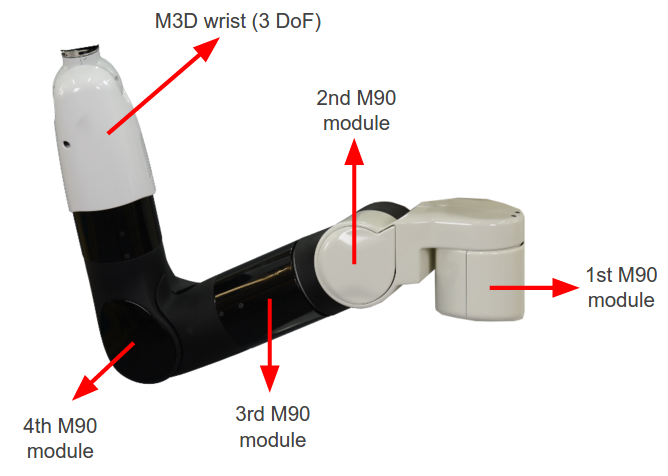
\includegraphics[width=\linewidth]{figures/Arm.png}
    \caption{The 7-DOF arm with its four M90 modules and 3-DOF wrist.
             Image courtesy of PAL Robotics.}
    \label{fig:arm_torso}
  \end{minipage}
  \hfill
  \begin{minipage}{0.48\textwidth}
    \centering
    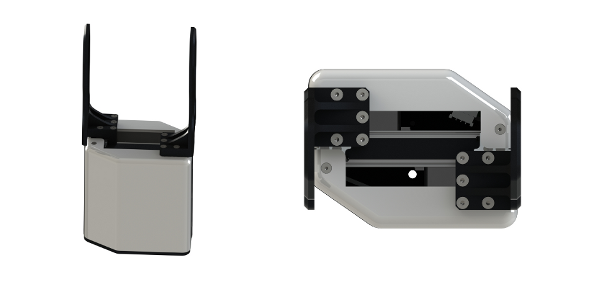
\includegraphics[width=\linewidth]{figures/Parallel_gripper.png}
    \caption{The PAL parallel two-finger gripper.
             Image courtesy of PAL Robotics.}
    \label{fig:gripper_head}
  \end{minipage}
\end{figure}

The robot's \textbf{head} carries the main perception sensor: an \textbf{Asus
Xtion Pro Live} structured-light RGB-D camera that provides registered colour
and depth images at up to 30\,fps at $640\times480$ resolution
(Figure~\ref{fig:head_kinematics}).
The head itself has two degrees of freedom --- pan (horizontal rotation,
$\pm1.5$\,rad) and tilt (vertical angle, $-0.8$ to $+0.4$\,rad) --- which allows
the camera to survey a wide field around the robot during object search.

\begin{figure}[H]
  \centering
  \begin{minipage}{0.48\textwidth}
    \centering
    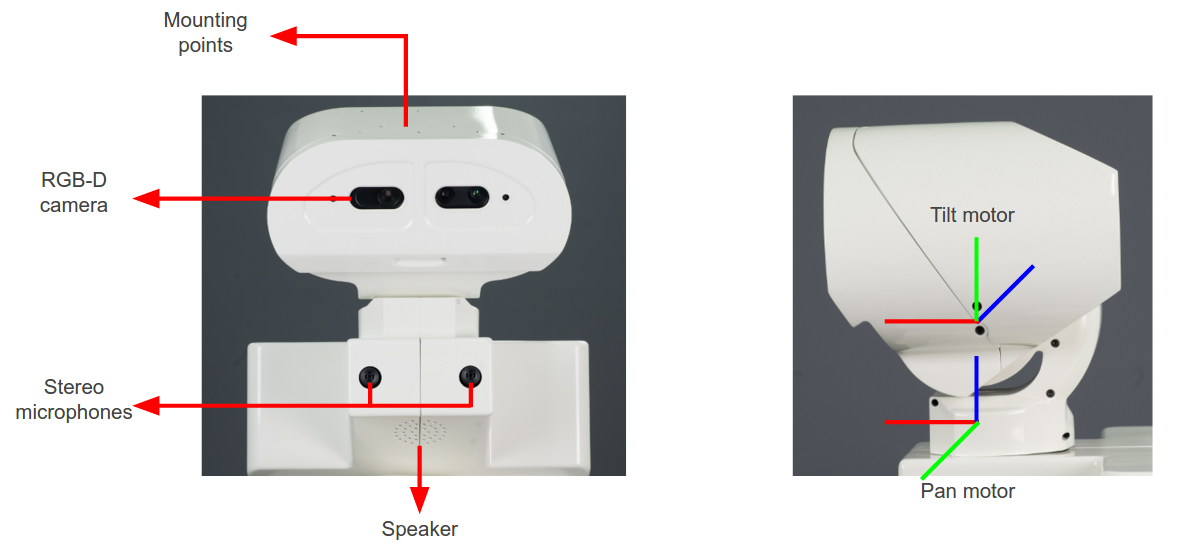
\includegraphics[width=\linewidth]{figures/Head_parts.png}
    \caption{TIAGo head assembly with the Xtion RGB-D camera, stereo microphone,
             and pan-tilt joints. Image courtesy of PAL Robotics.}
    \label{fig:head_kinematics}
  \end{minipage}
  \hfill
  \begin{minipage}{0.48\textwidth}
    \centering
    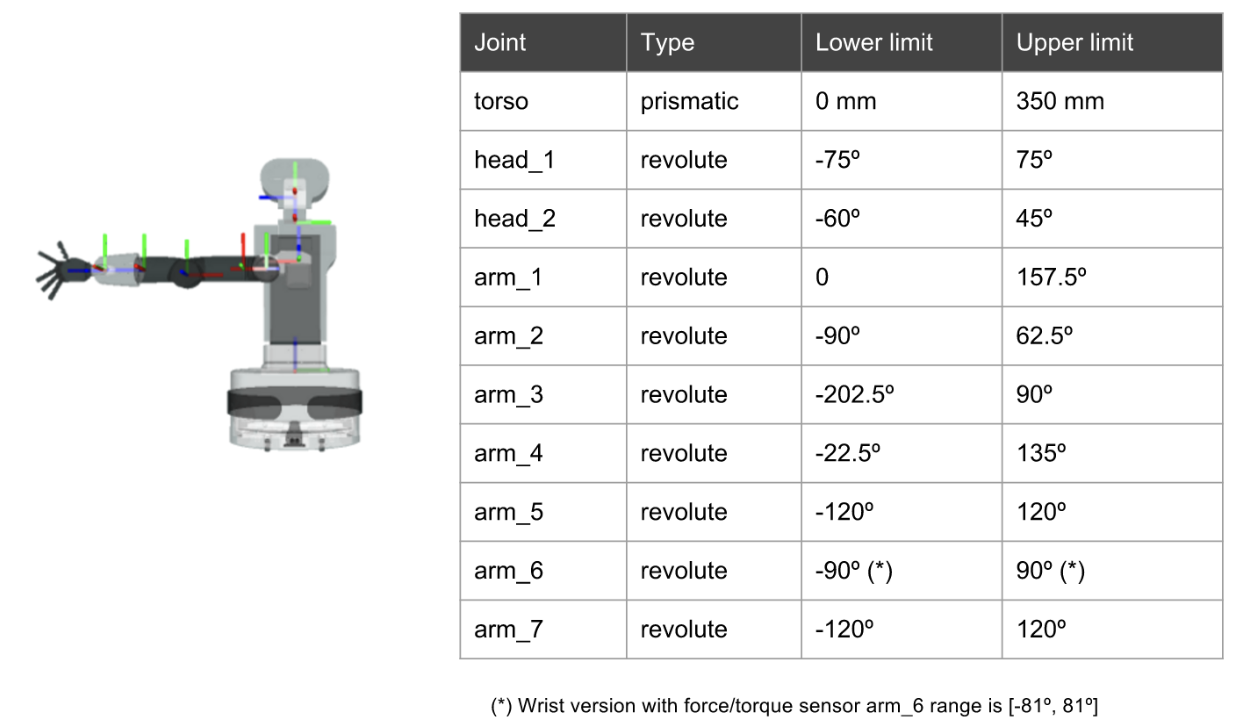
\includegraphics[width=\linewidth]{figures/kinematics.png}
    \caption{Upper-body kinematic structure and joint motion ranges.
             Image courtesy of PAL Robotics.}
    \label{fig:kinematics_detail}
  \end{minipage}
\end{figure}

A critical hardware constraint that shaped the entire software architecture is
that the robot's onboard computer runs \textbf{ROS Melodic under Ubuntu 18.04
inside a Docker container}, limiting the Python runtime to version 3.6.
This is incompatible with modern deep-learning inference frameworks (PyTorch,
ONNX Runtime, Ultralytics), all of which require Python 3.8 or later.
The architectural solution to this constraint is described in the next section.

% ============================================================
\section{Full System Architecture}
\label{sec:architecture}
% ============================================================

The TIAGo VLA agent is structured as a \textbf{four-layer heterogeneous system}
spanning a cloud reasoning service, a host machine running the neural network
inference, a Docker container executing all ROS and agent code, and the physical
robot hardware.
The central organising pattern is the \textbf{perceive-reason-act loop}: at each
cycle the agent captures an annotated image of the scene, sends it to a cloud
VLM that decides what to do next, executes the chosen skill on the robot, and
repeats until the task is complete.
Figure~\ref{fig:arch_full} shows the complete architecture with all components
and communication channels.

\begin{landscape}
\begin{figure}[p]
\centering
\begin{tikzpicture}[scale=0.69, transform shape,
  %--- node styles ---
  layer/.style={rectangle, rounded corners=6pt, draw=darkblue, very thick,
                minimum width=18cm, minimum height=1.0cm,
                fill=lightblue!12, font=\bfseries\small},
  box/.style={rectangle, rounded corners=4pt, draw=darkblue, thick,
              fill=white, minimum width=3.0cm, minimum height=0.85cm,
              align=center, font=\small},
  skillbox/.style={rectangle, rounded corners=3pt, draw=palgreen, thick,
                   fill=palgreen!10, minimum width=2.5cm, minimum height=0.75cm,
                   align=center, font=\footnotesize},
  hostbox/.style={rectangle, rounded corners=4pt, draw=codered, thick,
                  fill=codered!6, minimum width=4.5cm, minimum height=0.85cm,
                  align=center, font=\small},
  hwbox/.style={rectangle, rounded corners=4pt, draw=gray!60, thick,
                fill=gray!8, minimum width=2.8cm, minimum height=0.8cm,
                align=center, font=\small},
  boundary/.style={rectangle, rounded corners=8pt, dashed, thick},
  arr/.style={-{Stealth[length=7pt]}, thick, draw=darkblue},
  arrg/.style={-{Stealth[length=7pt]}, thick, draw=palgreen},
  arrr/.style={-{Stealth[length=7pt]}, thick, draw=codered},
  lbl/.style={font=\footnotesize\itshape, fill=white, inner sep=2pt},
]

%% ---- ROW 0: User ------------------------------------------
\node[box, fill=lightblue!25, minimum width=4cm] (user) at (0, 0)
  {\textbf{User}\\Voice / Text};

%% ---- ROW 1: Input processing ------------------------------
\node[box, fill=lightblue!20] (stt) at (-3.5, -2.2)
  {Whisper STT\\(local, 74M)};
\node[box, fill=lightblue!20] (txt) at (3.5, -2.2)
  {Text Input\\(typed command)};

%% ---- DOCKER BOUNDARY --------------------------------------
\draw[boundary, fill=lightblue!5, draw=darkblue!60]
  (-9.2, -3.0) rectangle (9.2, -14.5);
\node[font=\small\bfseries, text=darkblue!80] at (-6.5, -3.35)
  {Docker Container --- ROS Melodic / Python 3.6};

%% ---- ROW 2: Agent core ------------------------------------
\node[box, fill=lightblue!30, minimum width=5cm, minimum height=1.0cm]
  (agent) at (0, -4.5) {\textbf{EmbodiedAgent}\\orchestrator loop};

\node[box, minimum width=3.8cm] (vlm) at (-5.5, -6.5)
  {\textbf{VLMReasoner}\\Gemini 2.0 Flash\\(cloud API)};
\node[box, minimum width=3.8cm] (state) at (0, -6.5)
  {\textbf{StateManager}\\gripper state\\scene graph};
\node[box, minimum width=3.8cm, fill=codered!8] (safety) at (5.5, -6.5)
  {\textbf{Safety System}\\failure counter\\safe mode};

%% ---- ROW 3: Skills ----------------------------------------
\node[font=\small\bfseries, text=palgreen!80!black] at (0, -8.2) {Skill Library};
\node[skillbox] (sgrab)   at (-7.0, -9.0) {grab\_bottle};
\node[skillbox] (ssearch) at (-3.8, -9.0) {search\_with\_head};
\node[skillbox] (shand)   at (0.0, -9.0)  {handover\_to\_person};
\node[skillbox] (swave)   at (3.8, -9.0)  {wave\_hand};
\node[skillbox] (spose)   at (7.0, -9.0)  {go\_to\_safe\_pose};

%% ---- ROW 4: Perception ------------------------------------
\node[box, minimum width=5cm] (perc) at (-4.5, -11.0)
  {\textbf{PerceptionManager}\\RGB-D sync, RANSAC,\\5-frame averaging};

\node[box, minimum width=3.5cm] (moveit) at (3.5, -11.0)
  {\textbf{MoveIt}\\OMPL planning\\collision scene};

%% ---- HOST BOUNDARY ----------------------------------------
\draw[boundary, fill=codered!4, draw=codered!60]
  (-9.2, -14.5) rectangle (9.2, -17.0);
\node[font=\small\bfseries, text=codered!80] at (-6.0, -14.85)
  {Host Machine --- Python 3.10};
\node[hostbox] (yolo) at (0, -15.7)
  {\textbf{YOLO11n HTTP Service}\\port 5001 --- $\sim$18\,ms inference\\POST /detect $\rightarrow$ JSON detections};

%% ---- ROBOT HARDWARE  (below host) -------------------------
\draw[boundary, fill=gray!6, draw=gray!50]
  (-9.2, -17.0) rectangle (9.2, -19.8);
\node[font=\small\bfseries, text=gray!70] at (-6.5, -17.35)
  {TIAGo Robot Hardware --- ROS Action Servers};
\node[hwbox] (hw_arm)  at (-6.0, -18.5) {7-DOF Arm\\MoveIt / FJT};
\node[hwbox] (hw_grip) at (-2.0, -18.5) {Gripper\\open / close};
\node[hwbox] (hw_head) at (2.0,  -18.5) {Head 2-DOF\\pan / tilt};
\node[hwbox] (hw_base) at (6.0,  -18.5) {Mobile Base\\move\_base};

%% ---- ARROWS -----------------------------------------------
% User -> STT / Text
\draw[arr] (user.south west) -- node[lbl,left]{audio} (stt.north);
\draw[arr] (user.south east) -- node[lbl,right]{text} (txt.north);
% STT/Text -> Agent
\draw[arr] (stt.south)  -- ++(0,-0.5) -| node[lbl,above left]{command} (agent.north west);
\draw[arr] (txt.south)  -- ++(0,-0.5) -| node[lbl,above right]{command}(agent.north east);
% Agent <-> VLM
\draw[arr] (agent.south west) -- node[lbl,left]{image+state} (vlm.north);
\draw[arr] (vlm.north east)   -- node[lbl,right]{skill+rationale} (agent.south);
% Agent <-> State
\draw[arr,<->] (agent.south) -- (state.north);
% Agent <-> Safety
\draw[arr] (agent.south east) -- node[lbl,right]{failures} (safety.north);
\draw[arr] (safety.west) -- node[lbl,above]{block} (state.east);
% Agent -> Skills
\draw[arrg] (agent.south) -- ++(0,-0.9) -| (sgrab.north);
\draw[arrg] (agent.south) -- ++(0,-0.9) -| (ssearch.north);
\draw[arrg] (agent.south) -- ++(0,-0.9) -- (shand.north);
\draw[arrg] (agent.south) -- ++(0,-0.9) -| (swave.north);
\draw[arrg] (agent.south) -- ++(0,-0.9) -| (spose.north);
% Skills -> Perception
\draw[arr] (sgrab.south)   -- ++(0,-0.4) -| (perc.north);
\draw[arr] (ssearch.south) -- ++(0,-0.4) -| (perc.north);
\draw[arr] (shand.south)   -- ++(0,-0.4) |- (perc.north east);
% Skills -> MoveIt
\draw[arr] (sgrab.south)   -- ++(0,-0.4) -| (moveit.north);
\draw[arr] (shand.south)   -- ++(0,-0.4) -| (moveit.north);
% Perception <-> YOLO
\draw[arrr] (perc.south) -- ++(0,-0.6) node[lbl,right]{JPEG frame}
            -- ++(0,-0.6) -- (yolo.north west);
\draw[arrr] (yolo.north west) -- ++(0,0.6) node[lbl,left]{JSON detections}
            -- ++(0,0.6) -| (perc.south);
% MoveIt -> Arm/Gripper HW
\draw[arr] (moveit.south) -- ++(0,-0.5) -| (hw_arm.north);
\draw[arr] (moveit.south) -- ++(0,-0.5) -| (hw_grip.north);
% Perception -> Head HW
\draw[arr] (perc.south) -- ++(0,-1.2) -| (hw_head.north);
% Perception -> Base
\draw[arr, dashed] (moveit.south east) -- ++(0,-0.5) -| (hw_base.north);
% Camera -> Perception (feedback)
\draw[arr, dotted, draw=gray] (hw_head.north east) -- ++(1.5,0)
  -- ++(0,5.5) node[lbl,right]{RGB-D frames} -| (perc.north east);

\end{tikzpicture}
\caption{Full architecture of the TIAGo VLA agent system. The Docker container
  (blue) runs all ROS and agent code under Python~3.6. The host machine (red)
  runs the YOLO11n detection service under Python~3.10 and communicates via
  HTTP. Solid arrows indicate primary data flow; dashed arrows indicate
  navigation commands; dotted arrows indicate sensor feedback.}
\label{fig:arch_full}
\end{figure}
\end{landscape}

\subsection{Architectural Layers}

The diagram in Figure~\ref{fig:arch_full} is best read from top to bottom as a
layered decomposition of concerns, with the user at the top and the physical
robot hardware at the bottom.

\paragraph{User input layer.}
The user issues commands either by speaking into a microphone or by typing at
the terminal.
Spoken audio is routed through \textbf{Whisper STT} (74\,M parameters, running
locally on the laptop CPU), while typed commands bypass speech recognition
entirely.
Both paths produce a plain-text command string that is passed to the agent.

\paragraph{Docker container (Python 3.6, ROS Melodic).}
The innermost blue boundary encloses every component that depends on ROS.
The \textbf{EmbodiedAgent} is the orchestrator: it holds references to all
subsystems, drives the perceive-reason-act loop, and decides when a task is
complete.
Beneath it, three support modules run concurrently.
The \textbf{VLMReasoner} manages all communication with the Gemini API,
encoding images, maintaining conversation history, and parsing JSON responses.
The \textbf{StateManager} subscribes to ROS sensor topics and maintains a
structured, serialisable summary of the robot's state.
The \textbf{Safety System} tracks consecutive failure counts and enforces
safe-mode entry.
Below these, the \textbf{Skill Library} contains seven specialised skill
modules, each inheriting from a common abstract interface.
Two of those skills (\texttt{grab\_bottle} and \texttt{handover\_to\_person})
delegate perception work to the \textbf{PerceptionManager}, which handles
RANSAC-based 3-D localisation, and delegation of arm motion to
\textbf{MoveIt}, the ROS motion planner.

\paragraph{Host machine (Python 3.10).}
The red boundary encloses the \textbf{YOLO11n HTTP Service} --- the one
component that cannot run inside Docker because Ultralytics requires Python 3.8.
The service wraps the model in a minimal Flask server that accepts JPEG frames
via HTTP POST and returns JSON detection arrays.
It is architecturally decoupled from the ROS stack: it can be restarted,
swapped for a different model, or queried by any external tool without touching
the agent code.

\paragraph{Robot hardware (ROS action servers).}
The grey boundary represents the physical TIAGo hardware, accessible from the
Docker container exclusively through typed ROS interfaces.
The arm, gripper, head, and mobile base each expose ROS action servers
(\path{FollowJointTrajectory} for the arm and head;
\path{/parallel\_gripper\_controller} for the gripper;
\path{move\_base} for navigation).
The PAL \path{play\_motion} and \path{/tts} action servers provide higher-level
primitives (named motion trajectories and text-to-speech output) that are used
by the skill library.

\paragraph{Cloud (Google Gemini API).}
The VLMReasoner communicates outward through the Docker network to
Eden AI's \texttt{api.edenai.run} REST endpoint (which proxies to Gemini 2.0 Flash).
This cloud dependency is the single point that requires an internet connection
at runtime; all other system components run on local hardware.

\subsection{The Split-Process Design}

The separation between the Docker container and the host machine is the most
architecturally unusual aspect of the system.
It was originally forced by the Python 3.6 constraint: the Docker image
provided by PAL Robotics for TIAGo ships with Python 3.6 baked in, and
replacing it would break the ROS Melodic Python bindings.
Modern neural network inference frameworks (PyTorch, Ultralytics YOLO,
ONNX Runtime) all require Python 3.8 or later and refuse to install
under 3.6.

Rather than forking or patching the PAL image --- a fragile approach that would
need to be maintained across ROS updates --- the decision was taken to keep the
constraint and work around it architecturally.
The neural network is deployed on the host, which has a clean Python 3.10
environment, and the two processes communicate over the loopback network via HTTP.
Figure~\ref{fig:split_proc} illustrates the boundary.

\begin{figure}[H]
\centering
\begin{tikzpicture}[
  proc/.style={rectangle, rounded corners=6pt, draw=darkblue, thick,
               fill=lightblue!15, minimum width=5.5cm, minimum height=3.2cm,
               align=center},
  comp/.style={rectangle, rounded corners=4pt, draw=darkblue, thick,
               fill=white, minimum width=4.6cm, minimum height=0.65cm,
               align=center, font=\small},
  hostcomp/.style={rectangle, rounded corners=4pt, draw=codered, thick,
               fill=codered!8, minimum width=4.6cm, minimum height=0.65cm,
               align=center, font=\small},
  arr/.style={-{Stealth[length=6pt]}, thick},
  lbl/.style={font=\footnotesize, fill=white, inner sep=2pt},
]

% Docker process
\node[proc, draw=darkblue!60, fill=lightblue!10,
      minimum width=5.5cm, minimum height=4.2cm] (docker) at (-3.5,0) {};
\node[font=\small\bfseries, text=darkblue] at (-3.5, 1.6)
  {Docker (Python 3.6)};
\node[comp] at (-3.5,  0.7) {EmbodiedAgent};
\node[comp] at (-3.5, -0.1) {PerceptionManager};
\node[comp] at (-3.5, -0.9) {VLMReasoner};
\node[comp] at (-3.5, -1.7) {Skill Library};

% Host process
\node[proc, draw=codered!60, fill=codered!5,
      minimum width=5.5cm, minimum height=2.0cm] (host) at (3.5,0) {};
\node[font=\small\bfseries, text=codered] at (3.5, 0.8)
  {Host (Python 3.10)};
\node[hostcomp] at (3.5, 0.0) {YOLO11n (Ultralytics)};
\node[hostcomp] at (3.5,-0.8) {Flask HTTP server :5001};

% HTTP arrow
\draw[arr, draw=codered, very thick]
  (-1.55, -0.1) -- node[lbl, above]{POST /detect} node[lbl, below]{JPEG}
  (1.55, -0.1);
\draw[arr, draw=palgreen, very thick]
  (1.55, 0.3) -- node[lbl, above]{JSON detections} (- 1.55, 0.3);

\end{tikzpicture}
\caption{The split-process design: the ROS agent runs in Docker (Python~3.6)
  while the neural network runs on the host (Python~3.10), communicating via
  HTTP on the loopback interface.}
\label{fig:split_proc}
\end{figure}

What began as an unwanted engineering constraint turned out to be a clean
architectural separation.
The concerns are genuinely distinct: the Docker container handles all
real-time robot control (timing-critical ROS callbacks, motion planning,
joint commands), while the host handles GPU-accelerated inference.
Upgrading the detector from YOLO11n to a future model requires only
restarting the microservice on the host; the agent code in Docker is
untouched.
The HTTP interface is also trivially testable: any developer can POST
a JPEG to \texttt{localhost:5001/detect} and inspect the JSON response
without launching ROS.

\subsection{Component Inventory and Interfaces}

Table~\ref{tab:components} lists every software component in the system with
its physical location, programming environment, external interface, and
primary responsibility.

\begin{table}[H]
\centering
\caption{Component inventory: location, interface, and responsibility.}
\label{tab:components}
\small
\begin{tabularx}{\linewidth}{l l X}
\toprule
\textbf{Component} & \textbf{Location / Env.} & \textbf{Interface \& Responsibility} \\
\midrule
EmbodiedAgent      & Docker / Py 3.6  & Central orchestrator; drives perceive-reason-act loop \\
VLMReasoner        & Docker / Py 3.6  & REST POST to Gemini API; returns parsed JSON skill \\
StateManager       & Docker / Py 3.6  & Subscribes \path{/joint_states}, \path{/odom}; exposes \texttt{get\_state()} \\
PerceptionManager  & Docker / Py 3.6  & HTTP client to YOLO service; RANSAC localisation \\
Skill Library (7)  & Docker / Py 3.6  & BaseSkill interface; direct ROS action calls \\
Safety System      & Docker / Py 3.6  & Failure counter; SIGINT/SIGTERM handler \\
MoveIt             & Docker / Py 3.6  & OMPL motion planner; collision scene management \\
YOLO11n Service    & Host / Py 3.10   & Flask HTTP :5001; POST JPEG $\to$ JSON detections \\
Whisper STT        & Host / Py 3.10   & Local speech recognition; 74M Transformer model \\
Gemini 2.0 Flash   & Google Cloud     & REST API; multimodal reasoning, JSON output \\
TIAGo Arm          & Robot HW         & \path{/arm_controller/follow_joint_trajectory} action \\
TIAGo Gripper      & Robot HW         & \path{/parallel_gripper_controller/...} action \\
TIAGo Head         & Robot HW         & \path{/head_controller/follow_joint_trajectory} action \\
play\_motion       & Robot HW         & \path{/play_motion} action; named PAL trajectories \\
PAL TTS            & Robot HW         & \path{/tts} action; text-to-speech in English \\
Mobile Base        & Robot HW         & \path{/move_base} action; 2-D laser navigation \\
\bottomrule
\end{tabularx}
\normalsize
\end{table}

\subsection{Key ROS Topics and Data Flows}

Communication within the Docker container uses standard ROS mechanisms.
Table~\ref{tab:ros_topics} lists the ROS topics that carry sensor data
into the agent and monitoring data out of it.

\begin{table}[H]
\centering
\caption{Key ROS topics used by the agent.}
\label{tab:ros_topics}
\small
\begin{tabularx}{\linewidth}{l l X}
\toprule
\textbf{Topic} & \textbf{Direction} & \textbf{Content} \\
\midrule
\path{/xtion/rgb/image_raw}              & In  & Raw colour frames at 30\,fps ($640\times480$, BGR8) \\
\path{/xtion/depth_registered/image_raw} & In  & Registered depth frames, aligned to RGB frame \\
\path{/xtion/rgb/camera_info}            & In  & Intrinsic calibration: $f_x, f_y, c_x, c_y$ \\
\path{/joint_states}                     & In  & All joint positions including gripper fingers \\
\path{/mobile_base_controller/odom}      & In  & Odometry pose for base-location tracking \\
\path{/agent/camera_annotated}           & Out & Annotated frame with YOLO boxes and depths \\
\path{/agent/status}                     & Out & JSON status: current skill, rationale, state \\
\bottomrule
\end{tabularx}
\normalsize
\end{table}

The \emph{annotated frame} on \path{/agent/camera\_annotated} is the same
image that gets sent to the VLM: YOLO bounding boxes are drawn on the raw
colour frame, with class labels and estimated depths overlaid.
Publishing this on a ROS topic makes it available both to RViz and to the
MJPEG stream on port 8080, so the operator can verify in real time exactly
what the VLM ``sees'' at each reasoning step.
The \path{/agent/status} topic carries a JSON string that is simultaneously
served as a live endpoint on port 8081, enabling the web visualisation
dashboard to display the current skill name, the VLM's stated rationale,
the full state dictionary, and the consecutive failure counter.

% ============================================================
\section{The Perceive-Reason-Act Loop}
\label{sec:loop}
% ============================================================

Every task begins with a command from the user --- either spoken into a USB
microphone or typed at the terminal.
Spoken audio is transcribed locally using \textbf{Whisper base} (74\,M
parameters), a transformer-based speech recognition model that runs in real
time on the laptop CPU and handles accented or lightly imperfect speech
significantly better than classical HMM-based systems.
The agent queries each available audio device in priority order, preferring
the robot's built-in stereo microphone before falling back to any USB audio
device; if no microphone is detected, it falls back to Google Cloud
Speech-to-Text via the \texttt{speech\_recognition} library.

Once the command text is available, the agent opens its \textbf{multi-step
execution loop}, shown in simplified form in Listing~\ref{lst:agent_loop}.
The loop is bounded by two hard limits: a maximum of \texttt{max\_steps = 5}
iterations per task (preventing runaway execution chains) and a
\texttt{max\_consecutive\_failures = 3} threshold that, once exceeded, triggers
a protective safe mode.

\begin{lstlisting}[language=Python, caption={Simplified perceive-reason-act loop in \texttt{EmbodiedAgent.execute\_task()}.}, label={lst:agent_loop}]
def execute_task(self, user_command):
  last_affordance_failure = {}
  last_skill = None

  for step in range(self.max_steps):          # hard limit: 5 steps

    # 1. Capture scene and run detection
    image, detections = self.perception.capture_and_detect()

    # 2. Assemble structured state context
    state = self.state_manager.get_state()

    # 3. Query VLM with image + state + previous failure feedback
    response = self.vlm.query(
      user_command, image, detections, state,
      affordance_failures=last_affordance_failure
    )
    skill_name = response['skill']
    params     = response['parameters']

    # 4. Affordance (precondition) check
    skill    = self.skill_registry[skill_name]
    ok, reason = skill.check_affordance(params, state)
    if not ok:
      last_affordance_failure[skill_name] = reason
      self.consecutive_failures += 1
      if self.consecutive_failures >= self.max_consecutive_failures:
        self._enter_safe_mode()
        return
      continue        # re-query VLM with failure injected

    # 5. Execute skill (blocking)
    last_affordance_failure = {}
    self.consecutive_failures = 0
    skill.execute(params)
    self.state_manager.update(skill_name, success=True)

    # 6. Task completion check
    if response.get('task_complete') or skill_name == last_skill:
      break
    last_skill = skill_name
\end{lstlisting}

\subsection{Affordance Failure Injection}

The most important design detail in the loop is the
\textbf{affordance failure injection} mechanism (lines 14 and 25 of
Listing~\ref{lst:agent_loop}).
When a skill's precondition check fails --- for example, because the VLM
selected \texttt{grab\_bottle} but the gripper is already closed ---
the failure reason string is stored in the \texttt{last\_affordance\_failure}
dictionary, which is passed to the \emph{next} VLM call.
The \texttt{VLMReasoner.query()} method serialises this dictionary and appends
it to the user prompt as a dedicated section:

\begin{mdframed}[style=promptbox]
\texttt{FAILED PRECONDITIONS (do NOT retry these):}\\
\texttt{~~grab\_bottle: gripper already closed ---}\\
\texttt{~~~~~~~~~~~~~~~~choose handover\_to\_person or open\_gripper first}
\end{mdframed}

This closed-loop \emph{inner monologue} feedback --- structurally equivalent to
the Inner Monologue approach of \cite{huang2022inner} --- transforms the VLM
from a brittle one-shot oracle into a self-correcting planner.
Without it, an incorrect VLM decision would simply repeat on the next iteration
and exhaust all allowed steps.
With it, the failure message is injected into the context, and the model
typically corrects itself within one additional iteration.

\subsection{Task Completion Heuristics}

Two complementary conditions terminate the loop.
The primary condition is that the VLM sets \texttt{task\_complete: true} in its
JSON response.
The secondary condition (line 32) encodes a practical heuristic: if the model
selects the same skill on two consecutive steps, the task is considered done.
This catches cases where \texttt{task\_complete} is accidentally omitted after
a successful handover, which would otherwise cause the agent to attempt a second
handover of an already-released object.

% ============================================================
\section{Perception Pipeline}
\label{sec:perception}
% ============================================================

The perception subsystem solves two distinct problems: detecting \emph{what}
objects are in the scene and localising \emph{where} they are in 3-D space.
These are handled by two tightly coupled modules.

\subsection{YOLO11n Object Detection Microservice}

Semantic detection uses \textbf{YOLO11n}, the nano variant of Ultralytics'
latest architecture, running as an HTTP microservice on the host machine's
Python 3.10 environment.
The container sends a raw JPEG frame and receives a JSON array of detections
within approximately 18\,ms --- fast enough for a 15\,fps annotation pipeline.

\begin{lstlisting}[language={}, numbers=none,
    caption={YOLO11n microservice HTTP interface (port 5001).}]
POST http://<HOST_IP>:5001/detect
Content-Type: image/jpeg
X-Classes: bottle,person         # optional server-side class filter

Response (JSON array):
[
  {"class_name": "bottle",  "confidence": 0.87,
   "bbox": [u1, v1, u2, v2]},
  {"class_name": "person",  "confidence": 0.94,
   "bbox": [u1, v1, u2, v2]}
]
\end{lstlisting}

The optional \texttt{X-Classes} header filters detections server-side, which
reduces the JSON payload and avoids exposing irrelevant classes to the VLM.
The service is stateless and restartable independently of the ROS stack, giving
a clean separation of concerns between the AI inference layer and the robot
control layer.

\begin{sloppypar}
YOLO11n was selected over open-vocabulary alternatives
(YOLO-World~\cite{cheng2024yoloworld}, OwlViT~\cite{minderer2022owlvit},
Grounding DINO~\cite{liu2023gdino}) after empirical benchmarking on the
deployment hardware showed that those models required 150--500\,ms per frame
on CPU --- prohibitive for real-time robot control.
The trade-off is that YOLO11n is limited to the 80 COCO classes, but this
covers all objects the agent is currently expected to manipulate (bottles,
cups, bowls, persons).
Table~\ref{tab:yolo_micro} summarises the models evaluated.
\end{sloppypar}

\begin{table}[H]
\centering
\caption{Object detection models evaluated for this deployment.}
\label{tab:yolo_micro}
\small
\begin{tabular}{llll}
\toprule
\textbf{Model} & \textbf{Runtime} & \textbf{CPU infer.} & \textbf{Decision} \\
\midrule
YOLOv4-tiny   & Docker (cv2.dnn)  & $\sim$50\,ms  & Early versions \\
YOLO-World    & Host Py 3.10     & $\sim$150\,ms & Too slow \\
YOLOE-26s-seg & Host Py 3.10     & $\sim$300\,ms & Too slow \\
YOLO11n       & Host microservice & $\sim$18\,ms  & \textbf{Chosen} \\
\bottomrule
\end{tabular}
\normalsize
\end{table}

\subsection{3-D Object Localisation via RANSAC Cylinder Fitting}

Knowing that a bottle exists at pixel coordinates is not sufficient for
grasping --- the arm needs a 3-D position in the robot's base frame.
The localisation pipeline begins by back-projecting the YOLO bounding box onto
the registered depth image from the Xtion sensor.
For each pixel $(u, v)$ inside the bounding box with a valid depth value $d$,
the corresponding 3-D point in camera coordinates is:
\begin{equation}
  \mathbf{p}_{\text{cam}} =
  \begin{pmatrix}
    \dfrac{(u - c_x)\,d}{f_x} \\[6pt]
    \dfrac{(v - c_y)\,d}{f_y} \\[6pt]
    d
  \end{pmatrix}
\end{equation}
where $(f_x, f_y, c_x, c_y)$ are the camera intrinsics read from the
\path{/xtion/rgb/camera_info} topic.

This yields a 3-D point cloud of the object's visible surface.
Rather than taking the raw centroid (which is biased towards the object's
widest face), we fit a cylinder to the cloud in the $XY$ plane using
\textbf{RANSAC}~\cite{schnabel2007ransac}, as formalised in
Algorithm~\ref{alg:ransac}.

\begin{algorithm}[H]
\caption{RANSAC cylinder fitting for 3-D object localisation}
\label{alg:ransac}
\DontPrintSemicolon
\KwIn{Point cloud $\mathcal{P} = \{(x_i, y_i, z_i)\}$; $N_{\text{iter}} = 300$; threshold $\tau = 0.015$\,m; radius range $[r_{\min}, r_{\max}] = [0.015, 0.06]$\,m; $N_{\min\text{pts}} = 15$; $N_{\min\text{inl}} = 8$}
\KwOut{Best cylinder centre $(\hat{x}, \hat{y})$, radius $\hat{r}$; object top $\hat{z}$}
\If{$|\mathcal{P}| < N_{\min\text{pts}}$}{
  \Return{failure: insufficient depth coverage}\;
}
$\text{best\_inliers} \gets \emptyset$\;
\For{$i \gets 1$ \KwTo $N_{\text{iter}}$}{
  Sample 3 random points $\{p_1, p_2, p_3\} \subset \mathcal{P}$\;
  Fit circle $(x_c, y_c, r)$ to $XY$ projections of $\{p_1, p_2, p_3\}$\;
  \If{$r \notin [r_{\min}, r_{\max}]$}{\textbf{continue}\;}
  $\mathcal{I}_i \gets \{p \in \mathcal{P} : \bigl|\sqrt{(p_x-x_c)^2+(p_y-y_c)^2} - r\bigr| < \tau\}$\;
  \If{$|\mathcal{I}_i| > |\text{best\_inliers}|$}{
    $\text{best\_inliers} \gets \mathcal{I}_i$\;
  }
}
\If{$|\text{best\_inliers}| < N_{\min\text{inl}}$}{
  \Return{failure: too few inliers}\;
}
Refine $(\hat{x}, \hat{y}, \hat{r})$ by algebraic least-squares on
$\text{best\_inliers}$ (minimise $\sum_i (\sqrt{\Delta x_i^2+\Delta y_i^2} - r)^2$)\;
$\hat{z} \gets \min\{p_z : p \in \mathcal{P},\; p_v < v_{\min} + \tfrac{1}{4}(v_{\max}-v_{\min})\}$\quad (object top)\;
\Return{$(\hat{x}, \hat{y}, \hat{z})$, $\hat{r}$, inlier\_ratio $= |\text{best\_inliers}|/|\mathcal{P}|$}
\end{algorithm}

After each successful RANSAC fit, a \textbf{frame quality check} is applied:
if the inlier ratio falls below 0.30, the frame is discarded as unreliable.
To further suppress single-frame depth jitter from the Xtion's structured-light
pattern, the 3-D estimate is averaged over \textbf{five consecutive
high-quality frames}:
\begin{equation}
  (\hat{x},\hat{y},\hat{z}) =
  \frac{1}{5}\sum_{i=1}^{5}(x^{(i)},y^{(i)},z^{(i)})
\end{equation}
In practice this reduces the dominant positioning error from
$\sim$15\,mm (single frame) to below 5\,mm for a stationary object ---
well within the tolerance required for the gripper to close around a 500\,ml
bottle.

\subsection{Coordinate-Frame Management under Python 3.6}

A subtle implementation constraint is that the \texttt{tf2\_ros} Python
bindings require Python~3.8 or later; they are unavailable inside the
Docker container.
The solution is to obtain the camera-to-base transform once per grasp attempt
by spawning a subprocess:

\begin{lstlisting}[language=Python, numbers=none]
result = subprocess.check_output(
  ['rosrun', 'tf', 'tf_echo',
   'base_footprint', 'xtion_rgb_optical_frame'],
  timeout=5
)
# Parse translation + quaternion with regex
\end{lstlisting}

The output is parsed with a regular expression to extract the translation
vector and rotation quaternion.
This approach adds approximately 120\,ms per grasp attempt --- negligible
compared with the several seconds required for arm motion --- and has the
advantage of working without any native Python bindings.

% ============================================================
\section{Vision-Language Reasoning}
\label{sec:vlm}
% ============================================================

The VLM is the cognitive centre of the system: it observes an image and the
current context, then decides which action to take next.
This section describes all aspects of the VLM integration, from the API
communication layer to prompt design and failure handling.

\subsection{Model Selection and API Integration}

We chose \textbf{Google Gemini 2.0 Flash} after comparing it with GPT-4o and
locally-hosted LLaVA~1.6 on three criteria: inference latency (each agent step
blocks on the API response), instruction-following reliability (the model must
always produce valid JSON), and cost (the agent may invoke the VLM five or more
times per task).
Gemini 2.0 Flash consistently produced valid JSON on the first attempt,
responded in 1--4\,s, and cost approximately \$0.005 per call --- significantly
cheaper per image than GPT-4o.

The model is accessed via the \textbf{Generative Language REST API} rather than
the Python SDK (which requires Python~3.8):

\begin{lstlisting}[language={}, numbers=none,
    caption={REST API endpoint for Gemini 2.0 Flash via Eden AI.}]
POST https://api.edenai.run/v3/llm/chat/completions
Authorization: Bearer <EDENAI_API_KEY>
Content-Type: application/json
Body: {"model": "google/gemini-2-0-flash", "messages": [...], "max_tokens": 300}
\end{lstlisting}

The \texttt{VLMReasoner} class implements 3 automatic retries with exponential
back-off on HTTP errors.
If all retries fail or the response cannot be parsed as valid JSON (after
stripping any markdown code fences the model may accidentally include), the
reasoner returns a safe fallback: \texttt{\{"skill": "go\_to\_safe\_pose", ...
\}}.
This ensures that a transient network failure degrades gracefully to a safe arm
pose rather than an uncontrolled state.

\subsection{Image Encoding and Cost Optimisation}

Sending raw camera frames to the API would be both slow and expensive.
Before encoding, each image is resized so that its longest dimension does not
exceed \textbf{640 pixels} and re-compressed at \textbf{JPEG quality 85}:

\begin{lstlisting}[language=Python, numbers=none]
def encode_image(pil_image, max_size=640, quality=85):
  w, h = pil_image.size
  if max(w, h) > max_size:
    scale = max_size / max(w, h)
    pil_image = pil_image.resize(
      (int(w*scale), int(h*scale)), Image.LANCZOS)
  buffer = io.BytesIO()
  pil_image.save(buffer, format='JPEG', quality=quality)
  return base64.b64encode(buffer.getvalue()).decode('utf-8')
\end{lstlisting}

This reduces the per-image payload from $\sim$900\,KB (raw $640\times480$ RGB)
to approximately 35--50\,KB, cutting API transfer cost and latency without
meaningfully degrading the model's visual understanding for manipulation
tasks.

\subsection{Prompt Design}

The system prompt is the most important single engineering artefact in the
project: it defines the model's persona, its available actions, its output
contract, and the behavioural rules that prevent common failure modes.

\begin{mdframed}[style=promptbox]
\small
\textbf{SYSTEM PROMPT (condensed)}\\[4pt]
You are the cognitive controller of TIAGo, a PAL Robotics mobile manipulator.
Your role: observe the camera image, analyse the scene, and select the next
skill to execute.\\[4pt]
\textbf{Available skills:}\\
\texttt{grab\_bottle} | \texttt{search\_with\_head} |
\texttt{handover\_to\_person}\\
\texttt{wave\_hand} | \texttt{open\_gripper} | \texttt{close\_gripper} |
\texttt{go\_to\_safe\_pose}\\[4pt]
\textbf{Current state injected here:}\\
\texttt{gripper: open | base\_location: table}\\
\texttt{detected: [bottle @(0.3m, 0.1m), person @(1.5m)]}\\
\texttt{history: [grab\_bottle(success), ...]}\\[4pt]
\textbf{Output --- respond ONLY with valid JSON, no markdown, no prose:}\\
\texttt{\{"skill": "...", "parameters": \{...\}, "rationale": "...",}\\
\texttt{~"task\_complete": false\}}\\[4pt]
\textbf{Rules:} Never retry a skill listed in FAILED PRECONDITIONS.
Search before grasping an invisible object. If gripper is already closed,
do not attempt another grasp. Set \texttt{task\_complete: true} when done.
Express reasoning in \texttt{rationale} before choosing an action.
\end{mdframed}

The strict output constraint (\emph{``Respond ONLY with valid JSON, no
markdown, no prose''}) was essential.
Early iterations without this constraint produced free-text replies that
required fragile regex parsing and failed roughly 20\% of the time.
The current design reduces parse failures to negligible levels.

\subsection{Conversation History and Rolling Context}

The VLMReasoner maintains a \textbf{rolling 20-turn dialogue history}
(10 user + 10 model turns).
This history is included verbatim in every API call, giving the model
persistent memory of the task's progress: which skills executed successfully,
which objects were detected in previous frames, and which preconditions
previously failed.
When the history reaches 20 turns, the oldest pair is dropped in a FIFO
fashion to keep the context within the API's token limit.

\subsection{Post-Execution Verification}

After each skill execution, an optional \textbf{visual verification} step
sends two images --- a ``before'' snapshot captured just before the skill
and an ``after'' snapshot captured immediately after --- to the VLM with
a verification prompt.
The model returns a JSON object:
\begin{lstlisting}[language=JSON, numbers=none]
{"success": true,
 "observation": "Gripper closed around bottle, arm raised.",
 "issue": null}
\end{lstlisting}

This verification step is not on the critical execution path (failures do not
abort the task) but is logged for analysis and surfaced in the live
visualisation dashboard.

% ============================================================
\section{Manipulation and Grasping}
\label{sec:manipulation}
% ============================================================

Grasping is the most mechanically demanding capability in the system and the
part that required the most iterative development.
The final pipeline (version 5) went through five distinct design revisions,
each addressing a specific failure mode found during real-robot testing.

\subsection{From v1 to v5: An Iterative Journey}

\textbf{Version 1} used a simple MoveIt Cartesian goal directly in the robot's
base frame, relying on YOLO bounding-box centroids for the 3-D position.
It produced a working prototype, but single-frame depth noise caused the arm
to miss the object by 2--4\,cm, and the gripper had no calibrated offset
relative to the arm tool link.

\textbf{Version 2} addressed noise by introducing 5-frame temporal averaging
of depth estimates and added proper frame alignment between camera and base
using ROS TF.
This halved positioning errors but still relied on raw point-cloud centroids.

\textbf{Version 3} integrated the PAL parallel gripper with hand-calibrated
mechanical offsets measured using an interactive calibration script
(\texttt{calibrate\_grasp\_interactive.py}).
This brought the gripper reliably above the object centre, but Cartesian IK
failures near the table surface limited robustness.

\textbf{Version 4} replaced bounding-box centroids with RANSAC cylinder
fitting, exploiting the object's geometry for a more accurate and robust
centre estimate.
This dramatically improved accuracy for thin cylindrical objects (bottles)
and reduced false grasp attempts caused by centroid bias.

\textbf{Version 5} addressed the remaining IK failures by replacing the
Cartesian final-approach path with the \textbf{torso-descent} vertical
approach described below.

\subsection{The v5 Grasping Pipeline}

The complete v5 grasp sequence is as follows.

\begin{enumerate}[noitemsep]
  \item \textbf{Orient head.}
        Tilt the head to $-0.5$\,rad (looking down at the table), reading the
        current pan angle from \path{head_1_joint} on \path{/joint_states}
        to preserve the lateral direction already pointing at the object.

  \item \textbf{Unfold arm.}
        Command \texttt{play\_motion(``pregrasp\_bottle'')} to move the arm
        from its tucked rest configuration to a ready pose that clears
        the torso and base.

  \item \textbf{Open gripper.}
        Issue an open command via the gripper action server.

  \item \textbf{Record TF transform.}
        Obtain the camera-to-base transform once via \texttt{rosrun tf
        tf\_echo} (Section~\ref{sec:perception}).

  \item \textbf{Run 5-frame RANSAC localisation.}
        Collect five consecutive high-quality RANSAC fits and average them
        to obtain $(\hat{x}, \hat{y}, \hat{z})$ in the base frame.

  \item \textbf{Build collision scene.}
        Add two collision objects to MoveIt: a table box
        ($0.8\times1.2\times0.02$\,m centred 1\,cm below the estimated
        surface) and a cylindrical object placeholder with radius
        $(\hat{r} + 0.01)$\,m.

  \item \textbf{Move arm above object.}
        Command MoveIt with a \texttt{PoseStamped} goal positioned
        \texttt{descent = 0.20}\,m above the estimated grasp height,
        with the gripper oriented downward.

  \item \textbf{Torso descent.}
        Lower the torso joint from its current position to bring the
        gripper exactly to the grasp height.
        Because the torso is a world-Z-aligned prismatic joint, this
        guarantees a straight vertical trajectory with no IK computation.

  \item \textbf{Close gripper and lift.}
        Close the gripper with a maximum current limit of
        \textbf{0.35\,A} (preventing damage to soft objects), then raise
        the torso to lift the object 5\,cm off the table surface.
\end{enumerate}

\subsection{Calibrated Grasp Parameters}

The pre-grasp goal pose is expressed relative to the RANSAC-estimated object
centre using empirically calibrated offsets measured during development.
Table~\ref{tab:grasp_params} lists the final calibrated values.

\begin{table}[H]
\centering
\caption{Empirically calibrated v5 grasp parameters.}
\label{tab:grasp_params}
\small
\begin{tabularx}{\linewidth}{l p{3.8cm} X}
\toprule
\textbf{Parameter} & \textbf{Value} & \textbf{Description} \\
\midrule
Forward offset $\Delta x$    & $0.19$\,m    & Gripper to object centre along base-X \\
Lateral offset $\Delta y$    & $0.05$\,m    & Correction for gripper-to-tool-link asymmetry \\
Vertical offset $\Delta z$   & $0.0361$\,m  & Height of gripper fingers above object top \\
Descent distance             & $0.20$\,m    & Torso travel for final vertical approach \\
Gripper orient.\ $q$         & $(-0.640,\,-0.080,$\newline$\phantom{(}-0.020,\,+0.764)$ & Quaternion $(x,y,z,w)$ for downward grasp \\
Max gripper current          & $0.35$\,A    & Current limit to protect soft objects \\
\bottomrule
\end{tabularx}
\normalsize
\end{table}

The orientation quaternion $(-0.640,\,-0.080,\,-0.020,\,+0.764)$ was determined
by commanding the arm to the desired downward-pointing pose in MoveIt's
interactive marker, reading back the wrist joint quaternion, and hard-coding it.
Small deviations from perfect vertical ($x=-1,\,y=z=0,\,w=0$) in the
$y$- and $z$-components reflect the mechanical asymmetry of the PAL gripper
attachment and were retained as measured.

\subsection{Visual Search: The 12-Position Head Sweep}

When the VLM selects \texttt{search\_with\_head} because the target object is
not visible, the robot executes a systematic head sweep across twelve pan/tilt
positions that cover the full reachable field of view around the robot's
current position.
At each position, the head settles for 2\,s (allowing the image to stabilise)
before querying the YOLO service.
The sweep terminates as soon as the target class is detected with
confidence $>$\,0.4, or returns failure if all twelve positions have been
scanned without a detection.
Table~\ref{tab:search_positions} lists the twelve positions in scan order.

\begin{table}[H]
\centering
\caption{Head sweep positions for \texttt{search\_with\_head} skill (12 positions in order).}
\label{tab:search_positions}
\small
\begin{tabular}{clrrp{4.5cm}}
\toprule
\textbf{\#} & \textbf{Name} & \textbf{Pan (rad)} & \textbf{Tilt (rad)} & \textbf{Field covered} \\
\midrule
1  & centre          &  0.0  &  0.00  & Straight ahead, horizontal \\
2  & centre\_down    &  0.0  & $-0.45$  & Straight ahead, looking down \\
3  & left            &  0.8  &  0.00  & Left quarter \\
4  & left\_down      &  0.8  & $-0.45$  & Left quarter, looking down \\
5  & far\_left       &  1.4  &  0.00  & Hard left \\
6  & far\_left\_down &  1.4  & $-0.45$  & Hard left, looking down \\
7  & right           & $-0.8$  &  0.00  & Right quarter \\
8  & right\_down     & $-0.8$  & $-0.45$  & Right quarter, looking down \\
9  & far\_right      & $-1.4$  &  0.00  & Hard right \\
10 & far\_right\_down & $-1.4$ & $-0.45$ & Hard right, looking down \\
11 & up              &  0.0  & $+0.30$ & Straight ahead, elevated \\
12 & centre (return) &  0.0  &  0.00  & Reset to forward gaze \\
\bottomrule
\end{tabular}
\normalsize
\end{table}

A key implementation detail is that the tilt command reads the current pan
value from \path{/joint_states} before issuing the new head goal.
This prevents the head from snapping to the centre pan on every tilt change,
which would miss objects to the side and produce jerky motion.

\subsection{Person Handover Skill}

The \texttt{handover\_to\_person} skill completes the full
``find -- grasp -- deliver'' task chain.
Its affordance condition requires that the gripper is closed (holding an object)
\emph{and} that a person class detection is present in the current frame.

The execution sequence is:

\begin{enumerate}[noitemsep]
  \item \textbf{Detect person region.}
        Extract the YOLO bounding box for the nearest ``person'' detection.
        The person's estimated body centre is taken as the midpoint of the
        bounding box's middle horizontal and lower-vertical thirds.

  \item \textbf{Estimate person depth.}
        Back-project the body-centre pixel through the Xtion depth image
        to obtain the person's approximate 3-D position in the base frame.

  \item \textbf{Clear the octomap.}
        Call the \path{/clear_octomap} service to remove stale voxels
        around the person's position so that MoveIt can plan a
        collision-free path to the handover pose.

  \item \textbf{Add person collision box.}
        Insert a $0.50 \times 0.50 \times 1.80$\,m box at the estimated
        person position in the MoveIt planning scene.
        This prevents the arm from swinging through the person during
        trajectory planning.

  \item \textbf{Plan and execute arm motion.}
        Command MoveIt to a handover pose at:
        \[
          \text{height} = \text{HANDOVER\_HEIGHT} = 0.85\,\text{m},
          \quad
          \text{reach} = \text{ARM\_REACH} = 0.62\,\text{m}
        \]
        oriented toward the estimated person direction.

  \item \textbf{Wait and release.}
        Announce ``\emph{Here you go!}'' via the PAL TTS action server,
        wait 4\,s for the person to take the object, then open the gripper.

  \item \textbf{Clean up.}
        Remove the person collision object from the planning scene and
        return the arm to the pre-grasp pose.
\end{enumerate}

The 4-second wait is intentional: releasing too early (before the person has
grasped the object) would drop it, while waiting indefinitely would stall
the loop.
In practice, 4\,s is sufficient for a person standing within reach to close
their hand around the object.

% ============================================================
\section{Agent Orchestration and Skill Library}
\label{sec:agent}
% ============================================================

The agent is implemented as a class (\texttt{EmbodiedAgent}) that holds
references to all subsystems: the perception manager, the VLM reasoner, the
state manager, and the skill registry.
At initialisation it connects to all ROS action servers, verifies that the
YOLO microservice is reachable, and loads the skill library.
If any critical component is unavailable the agent reports the problem and
exits rather than operating in a degraded mode.

\subsection{Skill Library Design}

Every skill inherits from an abstract \texttt{BaseSkill} class that enforces
a three-method interface:

\begin{lstlisting}[language=Python, numbers=none,
    caption={Abstract base class for all skills.}]
class BaseSkill(ABC):
  @abstractmethod
  def check_affordance(self, params, state) -> Tuple[bool, str]:
    """Return (True, '') if executable, (False, reason) if not."""

  @abstractmethod
  def execute(self, params) -> bool:
    """Execute the skill; return True on success."""

  @abstractmethod
  def get_description(self) -> str:
    """One-line human-readable description for the VLM prompt."""
\end{lstlisting}

This design means that adding a new skill requires only implementing three
methods; the agent loop, precondition checking, failure injection, and
state updates are all handled centrally.

Table~\ref{tab:skill_library} lists the nine skills in the current library
with their affordance conditions.

\begin{table}[H]
\centering
\caption{Skill library: names, preconditions, and actions.}
\label{tab:skill_library}
\begin{tabularx}{\linewidth}{lXX}
\toprule
\textbf{Skill} & \textbf{Precondition} & \textbf{Action} \\
\midrule
\texttt{grab\_bottle}       & Gripper open; bottle visible in frame
                             & v5 nine-step grasp pipeline \\
\texttt{search\_with\_head} & None (always executable)
                             & 12-position pan/tilt sweep \\
\texttt{handover\_to\_person} & Gripper closed; person visible in frame
                             & Arm reach to 0.85\,m, open gripper \\
\texttt{wave\_hand}         & None
                             & play\_motion(``wave'') trajectory \\
\texttt{open\_gripper}      & Gripper closed
                             & Open gripper action \\
\texttt{close\_gripper}     & Gripper open
                             & Close gripper action \\
\texttt{go\_to\_safe\_pose} & None
                             & Tuck arm, open gripper \\
\bottomrule
\end{tabularx}
\end{table}

\subsection{State Manager}

The \texttt{StateManager} provides the VLM with a structured, persistent view
of the robot's state between loop iterations.
It subscribes to two ROS topics:

\begin{sloppypar}
\begin{itemize}
  \item \path{/joint_states} --- to infer gripper state from the
        \texttt{parallel\_gripper\_right\_finger\_joint} position:
        below 0.005\,m the gripper is treated as \emph{open};
        above 0.015\,m it is \emph{closed}.
        Values in between indicate a transition in progress.

  \item \path{/mobile_base_controller/odom} --- to track the robot's
        approximate base location for context-aware skill selection.
\end{itemize}
\end{sloppypar}

On each call to \texttt{get\_state()}, the manager returns a dictionary
containing:
(1) the current gripper state,
(2) the estimated base location,
(3) the most recent five detected objects with their pixel bounding boxes,
(4) the last three entries of the task history in the form
    ``\texttt{[+] grab\_bottle}'' / ``\texttt{[-] grab\_bottle}'', and
(5) up to ten spatial relations inferred from the detection geometry.

\paragraph{Scene graph inference.}
Spatial relations are inferred from the pixel positions of YOLO detections.
Two objects are marked as \emph{near} if the distance between their bounding-box
centres is below 150\,px.
Objects whose centres lie within 50\,px vertically are inferred as being
\emph{on the same surface}, which the state manager reports as ``on table''
when all such objects are at a consistent height.
Left/right and above/below relations are added for all object pairs whose
bounding boxes do not overlap.
This gives the VLM a lightweight semantic scene description without requiring
an explicit 3-D map.

\subsection{Live Visualisation}

To facilitate debugging and demonstrations, the agent publishes two continuous
output streams.
The \textbf{annotated image} --- the same frame sent to Gemini, with bounding
boxes and estimated depths overlaid --- is published on
\path{/agent/camera_annotated} (ROS \texttt{sensor\_msgs/Image}, BGR8) and
streamed as MJPEG on port 8080.
A \textbf{JSON status packet} containing the current skill name, VLM rationale,
full state dictionary, and consecutive failure count is published on
\path{/agent/status} (ROS \texttt{std\_msgs/String}) and served as a live
JSON endpoint on port 8081.
Both streams are accessible in a standard web browser without installing any
additional software.

% ============================================================
\section{Safety Architecture}
\label{sec:safety}
% ============================================================

Safety was designed in from the start rather than added as an afterthought.
The system has three complementary layers: affordance gating (preventing
physically unsafe actions before they start), failure counting (detecting
repeated failures), and graceful shutdown (recovering to a known safe state
in response to any termination signal).

\subsection{Affordance Gating}

Every skill exposes a \texttt{check\_affordance} method that the agent calls
\emph{before} sending any motion command to the robot.
If the precondition returns false, the skill is not executed; instead, the
failure reason is injected into the next VLM prompt via the affordance failure
mechanism described in Section~\ref{sec:loop}.
This layer prevented several potentially damaging arm movements during early
development, including cases where the VLM attempted a second grasp with the
gripper already loaded with a bottle.

\subsection{Consecutive Failure Counting and Safe Mode}

\begin{sloppypar}
The agent tracks the number of consecutive affordance or execution failures
in a counter that resets to zero on any successful skill completion.
When the counter reaches \texttt{max\_consecutive\_failures}$\,=3$, the agent
calls \texttt{\_enter\_safe\_mode()}:
\end{sloppypar}

\begin{enumerate}[noitemsep]
  \item Set the \texttt{safe\_mode} flag to \texttt{True} (blocks all further
        skill dispatch).
  \item Execute \texttt{go\_to\_safe\_pose} unconditionally.
  \item Announce the failure via TTS: \emph{``I am having trouble. Please check
        my state.''}.
  \item Wait for an operator \texttt{reset} command before resuming.
\end{enumerate}

\subsection{Graceful Shutdown on Interrupt}

The agent registers handlers for both \texttt{SIGINT} (keyboard interrupt) and
\texttt{SIGTERM} (system termination) that call a
\texttt{\_safe\_shutdown()} method before exiting:

\begin{lstlisting}[language=Python, numbers=none,
    caption={Signal handler for safe shutdown.}]
def _safe_shutdown(self):
  try:
    self.skills['open_gripper'].execute({})    # release held object
    self.skills['go_to_safe_pose'].execute({}) # tuck arm
  finally:
    rospy.signal_shutdown('Agent terminated')
  sys.exit(0)
\end{lstlisting}

This ensures that the robot always ends in a safe, tucked pose regardless
of how the agent is stopped --- whether by the operator pressing Ctrl-C,
a deployment script sending SIGTERM, or a Python exception that propagates
to the top level.
In practice, this prevented the arm from being left in an extended position
(a significant hazard for nearby persons) on several occasions during
development.
